\documentclass{article}
\usepackage[utf8]{inputenc}

\title{Heapsort}
\author{Manuel Serna-Aguilera}
\date{}
\setlength{\parindent}{0pt}

\usepackage{natbib}
\usepackage{graphicx}
\usepackage{amsmath}
\usepackage{clrscode3e} % use this to better format pseudocode

\begin{document}

\maketitle

Heapsort is a neat sorting algorithm, its running time is $\Theta{(n \cdot \log_2{(n)})}$, like merge sort, but it also sorts in-place. It also uses a data structure called a heap, but heaps are also good for making efficient priority queues. 

\section*{Introduction to Heaps}
We can use an array to describe a (binary) heap, which is simply a nearly complete binary tree as seen in figure 1. By nearly complete it means the lowest level of the tree may or may not be completely full. The tree representation is just so we can better visualize the procedures we will perform on the array (a more accurate low-level view).
\\ \\
An array $A$ represents a heap and has two attributes:\\
\begin{itemize}
    \item $\attrib{A}{length}$: the length/size of the array.\\
    \item $\attrib{A}{heap-size}$: number of valid elements in $A$ such that\\$0 \leq \attrib{A}{heap-size} \leq \attrib{A}{length}$.
\end{itemize}

\begin{figure}[h!]
\centering
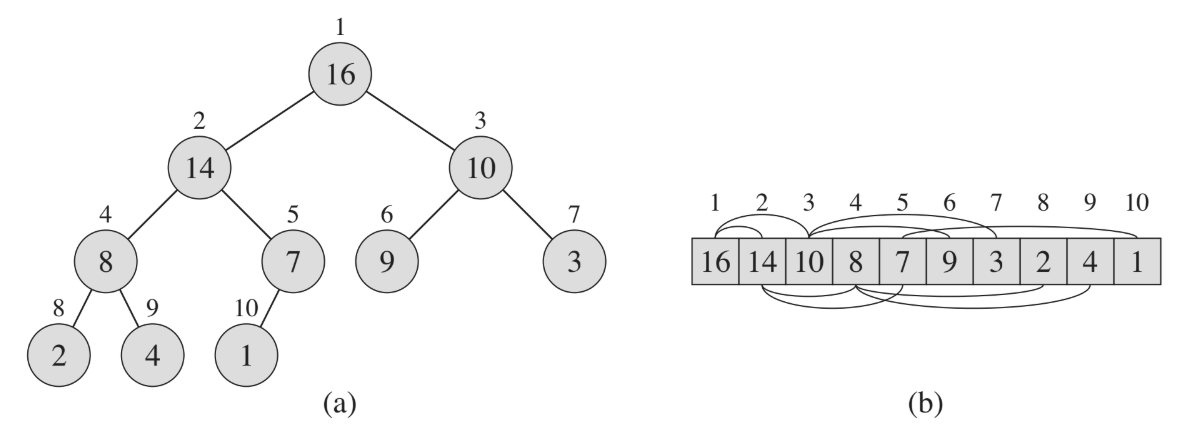
\includegraphics[scale=0.4]{heap_representation}
\caption{
  A max heap viewed as a \textbf{(a)} tree and \textbf{(b)} an array. Notice how labels and values in each node in the tree correspond to an index in the array. The height of the tree is $\Theta{(\log_2(n))}$.
}
\label{fig:heap_rep}
\end{figure}

The root of the tree is $A[1]$, and given an index $i$ of a node, we can compute:
\begin{codebox}
\Procname{\proc{parent}$(i)$}
\li \Return $\lfloor i/2 \rfloor$
\end{codebox}

\begin{codebox}
\Procname{\proc{left}$(i)$}
\li \Return $2i$
\end{codebox}

\begin{codebox}
\Procname{\proc{right}$(i)$}
\li \Return $2i + 1$
\end{codebox}

There are two kinds of binary heaps:
\begin{itemize}
    \item \textbf{Max heaps}: Must satisfy the \textbf{max heap} property, where the parent node at index $i$ is greater than or equal to its children. \\Formally, $A[\proc{parent}(i) \geq A[i]]$. With the largest node being the root. Heapsort utilizes max heaps.
    \\
    \item \textbf{Min heaps}: The opposite of the max heap property; the \textbf{min heap} property is satisfied when the parent node at index $i$ is less than or equal to its children. Formally, $A[\proc{parent}(i) \leq A[i]]$.
\end{itemize}

\section*{Max Heapify}
Max heapify is a procedure that maintains the max heap property. It assumes that the binary trees rooted at the left and right are max heaps, but the current node $i$ might be smaller than its children, thus potentially violating the max heap property.
\\ \\
If the max heap property is violated, then we must look at the left and right children of node $i$, and swap $i$ with whichever child has the bigger value. If the parent is already the largest, then the subtree rooted at $i$ is already a max heap, and the procedure terminates. Moving down a branch of the binary tree takes $O(\log_2{(n)})$, or $O(h)$, where the height of the tree is $ h = \log_2{(n)}$. Figure 2 illustrates an example of using the procedure on a single node, soon we will use it as a subroutine to build a max heap.

\newpage

\begin{codebox}
\Procname{$\proc{max-heapify}(A, i)$}
\li $l \gets \proc{left}(i)$
\li $r \gets \proc{right}(i)$
\li \If $l \leq \attrib{A}{heap-size}$ and $A[l] > A[i]$
\li     \Then
            $\id{largest} \gets l$ \Comment index of largest element is left child
\li     \Else
\li        $\id{largest} \gets i$ \Comment out of parent and left child, parent is larger
    \End
\li \Comment compare largest out of parent and left with the right (if it's in the valid heap)
\li \If $r \leq \attrib{A}{heap-size}$ and $A[r] > A[largest]$
\li     \Then
            $\id{largest} = r$ \Comment right child has the largest value
        \End
\li \If $\id{largest} \neq i$
\li     \Then 
            \Comment largest node was a child, keep going down to ensure max-heap property is not violated
\li         exchange $A[i]$ with $A[largest]$
\li         \proc{max-heapify}$(A, \id{largest})$
        \End
\end{codebox}
Since we go down a single branch in each call to $\proc{max-heapify}$, it costs $O(\log_2{(n)})$ time.

\begin{figure}[!ht]
\centering
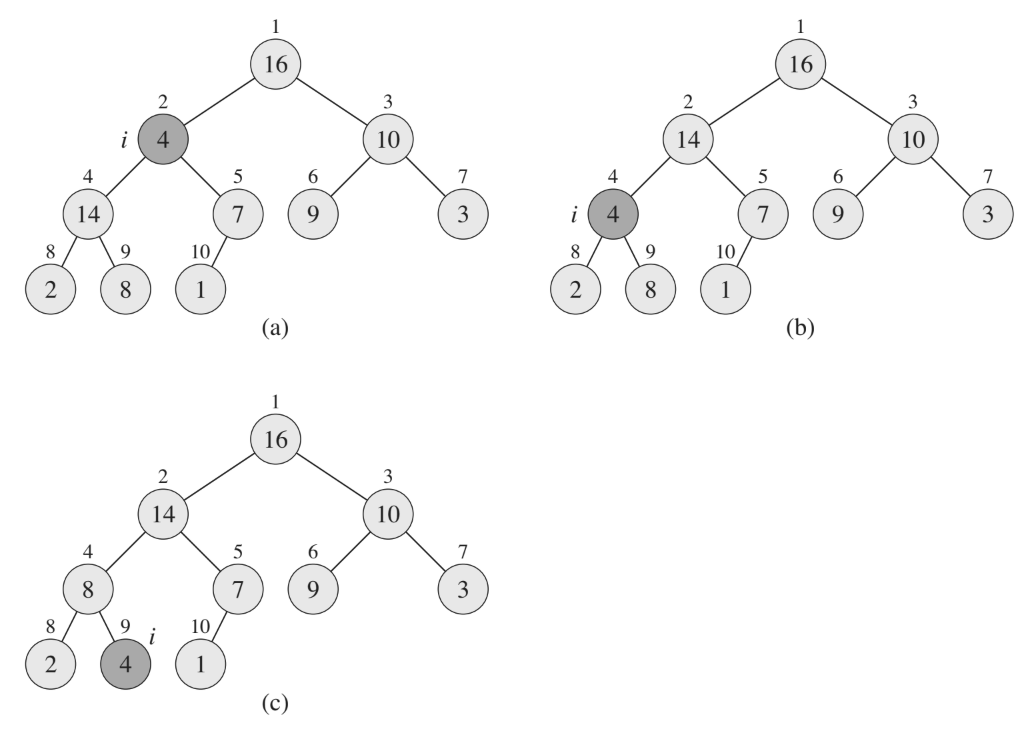
\includegraphics[scale=0.45]{max_heapify}
\caption{
  The process of calling $\proc{max-heapify}(A, 2)$. \textbf{(a)} Looking at $i=2$, which has a value of 4, is clearly smaller relative to both of its children. We will swap $i=2$'s 4 with its left child's ($i=4$) value of 14. \textbf{(b)} Now $i=4$ may violate the max heap property, and indeed it does, so we perform the swapping action again; swap the 4 with the 8 (the value of the right child). \textbf{(c)} Hooray! The procedure finishes as there are no children to compare with (in this case).
}
\label{fig:max_heapify_example}
\end{figure}

\newpage

\section*{Building a heap}
The $\proc{max-heapify}$ procedure can be used in a bottom-up manner to convert an array $A[1 \twodots n]$, where $n = \attrib{A}{length}$, into a max heap. The $\proc{build-max-heap}$ procedure starts at the last parent, and works its way up to the root, making every subtree a max heap.

\begin{codebox}
\Procname{$\proc{build-max-heap}(A)$}
\li $\attrib{A}{heap-size} \gets \attrib{A}{length}$ 
\li \For $i \gets \lfloor \attrib{A}{length}/2 \rfloor$ \Downto $1$
\li \Do
        $\proc{max-heapify}(A, i)$
    \End
\end{codebox}

Each call to $\proc{max-heapify}$ costs $O(\log_2(n))$ time, and $\proc{build-max-heap}$ makes $O(n)$ such calls. Thus, the running time is $O(n \cdot \log_2{(n)}$, but it can be bounded to be $O(n)$.

\newpage

Here is an example of the procedure $\proc{build-max-heap}(A)$ being called.

\begin{figure}[!ht]
\centering
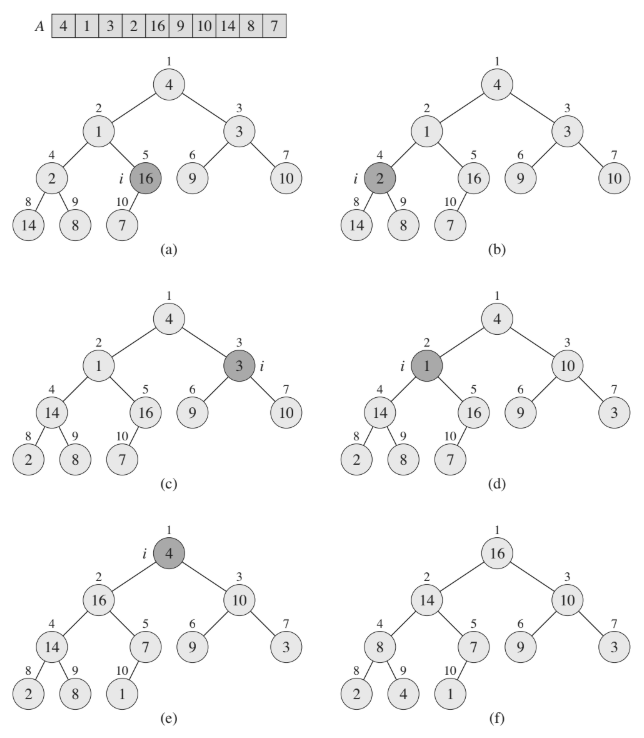
\includegraphics[scale=0.7]{build_max_heap}
\caption{
  \textbf{(a)} Start at $i=5$, it is larger than its left child, so no call to $\proc{max-heapify}$, move up to next parent. \textbf{(b)} At $i=4$, swap the values 2 and 14 to conform to the max-heap property, move up to the next parent. \textbf{(c)} At $i=3$, swap 3 and 10, move up to the next parent. \textbf{(d)} At $i=2$, swap 1 and 16. Now the value 1 is at $i=5$, but its left child at $i=10$ has a bigger value than it, so swap again. Now the subtree rooted at $i=2$ is a valid max heap. \textbf{(b)} At the root, we swap, 4 with 16, then 4 with 14, and then 4 with 8. \textbf{(f)} The final max heap.
}
\label{fig:build_heap}
\end{figure}

\newpage

\section*{Heapsort}
The heapsort algorithm starts by calling $\proc{build-max-heap}$ to build a max heap on the input array. We remove the value from the root by swapping it with the last value in the valid max heap, and place it at the end of the array. We then maintain the max heap and repeat the process for the max heap of size $n-1$ down to a heap of size 2. We then end up with an array with sorted values.

\begin{codebox}
\Procname{$\proc{heapsort}(A)$}
\li $\proc{build-max-heap}(A)$
\li \For $i \gets \attrib{A}{length}$ \Downto $2$
\li \Do
        exchange $A[1]$ with $A[i]$
\li     $\attrib{A}{heap-size} = \attrib{A}{heap-size}$
\li     $\proc{meax-heapify}(A, 1)$
    \End
\end{codebox}

Heapsort takes $O(n \cdot \log_2(n))$ time, since
\begin{itemize}
    \item $\proc{build-max-heap}$ takes $O(n)$ time.
    \item Each of the $n-1$ $\proc{max-heapify}$ calls takes time $O(\log_2(n))$.
\end{itemize}

% have heapsort figure in its own page
\newpage

\begin{figure}[!ht]
\centering
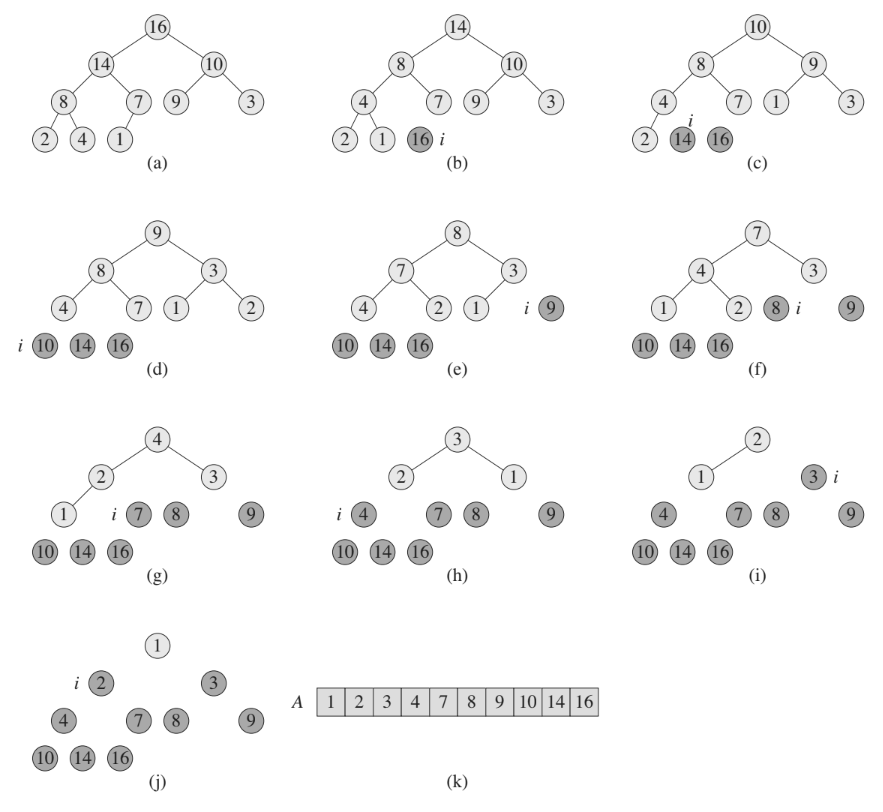
\includegraphics[scale=0.65]{heapsort}
\caption{
  The operation of $\proc{heapsort}$. \textbf{(a)} The max heap resulting after executing line 1. \textbf{(b) - (j)} The max heap after iterating through each node, notice how, visually, the larger values are swapped to be towards the bottom of the tree. \textbf{(k)} The array representation of the finished result (basically equivalent to (j)).
}
\label{fig:heapsort}
\end{figure}

\newpage

\section*{Priority Queues}
Even though heapsort is beat by quicksort pretty much every time, it is still very useful for making other data structures, like priority queues.
\\ \\
A \textbf{priority queue} is a data structure for maintaining a set $S$ of elements, each with an associated value called a \textbf{key}. A \textbf{max-priority queue} supports the following operations

% Use \item[] to exclude the bullet
\begin{itemize}
    \item[] $\proc{insert}(S, x)$ inserts the element $x$ into the set $S$, which is equivalent to the operation $S = S \cup \{x\}$. Has running time $O(\log_2(n))$.
    \item[] $\proc{maximum}(S)$ returns the element of $S$ with the largest key. Has running time $\Theta{(1)}$ since the root is the biggest value.
    \item[] $\proc{extract-max}(S)$ \textbf{removes} and returns the element of $S$ with the largest key. Has running time of $O(\log_2(n))$ since it performs only a constant amount of work on top of the $O(\log_2(n))$ time for calling $\proc{max-heapify}$.
    \item[] $\proc{increase-key}(S, x, k)$ increases the value of element $x$'s key to the new value $k$ such that \textit{old key} $\leq$ \textit{new key}. Has running time $O(\log_2(n))$. Refer to figure 5 at the end of the document to see the process visualized.
\end{itemize}
Do note that $\proc{max-heapify}$ and $\proc{heap-increase-key}$ can be thought of as maintaining the max heap property by going down and up a branch, respectively. This will be useful when writing the delete procedure.
\\ \\
Max-priority queues can be used for scheduling purposes. A \textbf{min-priority queue} supports the operations $\proc{insert}$, $\proc{minimum}$, $\proc{extract-min}$, and $\proc{decrease-key}$. A min-priority queue can be used in an event-driven simulator, where events are simulated in order of their time of occurrence (time acts as the key).

\newpage

Here is the pseudocode provided by the book.
%===================================
% Heap maximum
%===================================
\begin{codebox}
\Procname{$\proc{heap-maximum}(A)$}
\li \Return $A[i]$
\end{codebox}

%===================================
% Heap extract max
%===================================
\begin{codebox}
\Procname{$\proc{heap-extract-max}(A)$}
\li \If $\attrib{A}{heap-size} < 1$
\li \Then
        \Error ``heap underflow''
    \End
\li $\id{max} = A[1]$
\li \Comment Now adjust max-heap by propagating largest value to A[1]
\li $A[1] = A[\attrib{A}{heap-size}]$
\li $\attrib{A}{heap-size} = \attrib{A}{heap-size} - 1$
\li $\proc{max-heapify}(A, 1)$
\li \Return $\id{max}$
\end{codebox}

%===================================
% Heap increase key
%===================================
\begin{codebox}
\Procname{$\proc{heap-increase-key}(A, i, \id{key})$}
\li \If $\id{key} < A[i]$
\li \Then
        \Error ``new key is smaller than current key''
    \End
\li $A[i] = \id{key}$
\li \Comment Compare parent and current values, go up to satisfy max-heap property
\li \While $i >  1$ and $A[\proc{parent}(i)] < A[i]$
\li \Do
        exchange $A[i]$ with $A[\proc{parent}(i)]$
\li     $i = \proc{parent}(i)$
    \End
\end{codebox}

%===================================
% Max heap insert
%===================================
\begin{codebox}
\Procname{$\proc{max-heap-insert}(A, \id{key})$}
\li $\attrib{A}{heap-size} = \attrib{A}{heap-size} + 1$
\li $A[\attrib{A}{heap-size}] = -\infty$
\li $\proc{heap-increase-key}(A, \attrib{A}{heap-size}, key)$
\end{codebox}

%===================================
% Heap delete
%===================================
\begin{codebox}
\Procname{$\proc{heap-delete}(A, i)$}
\li swap $A[i]$ and $A[\attrib{A}{heap-size}]$
\li $\attrib{A}{heap-size} = \attrib{A}{heap-size} - 1$
\li \If $A[i] > A[\proc{parent}(i)]$
\li \Then
        $\proc{heap-increase-key}(A, i, A[i])$
    \End
\li \Else
\li \Then
        $\proc{max-heapify}(A, i)$ \Comment check if we need to stop or keep going down
    \End
\end{codebox}

For the $\proc{heap-delete}$ procedure, since we are going up or down a single branch of the binary tree, the running time is $O(\log_2(n))$. Note that in the call to $\proc{max-heapify}$, we check for which child branch to go down, and remember it also checks when to stop, so that is all we need to write.

% Note: the min-priority queue counterparts in the pseudocode file.

\newpage

\begin{figure}[!ht]
\centering
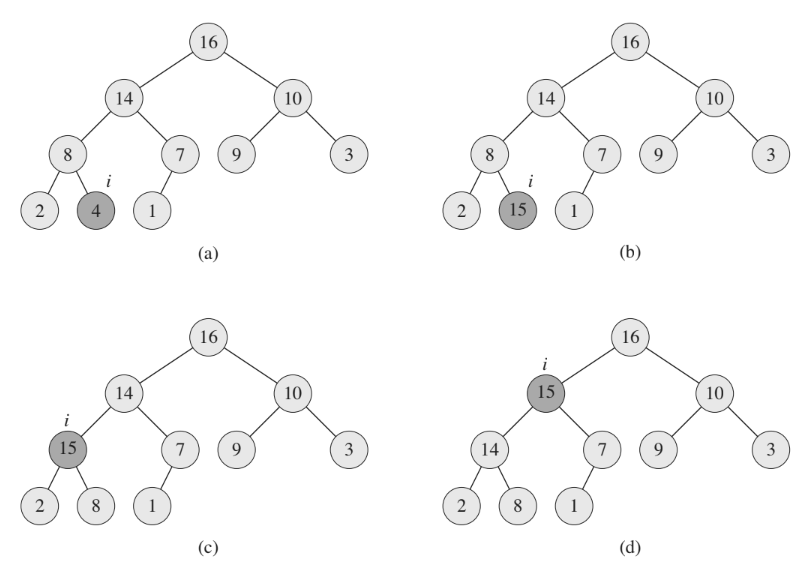
\includegraphics[scale=0.65]{heap_increase_key}
\caption{
  The process of calling $\proc{heap-increase-key}$. 
  \textbf{(a)} The procedure is called on $i$ whose key right now is 4.
  \textbf{(b)} The node's value is then increased to 15, the max heap property is clearly violated, we must now go up the binary tree to fix this.
  \textbf{(c)} Going up one level, 15 is not less than 14, the max heap property is still violated, thus we must keep going.
  \textbf{(d)} Final adjusted max heap, 15 is greater than each of its childrens' keys but less than its parent's key.
}
\label{fig:max-priority_queue}
\end{figure}

\end{document}
